% vim: set textwidth=78 autoindent:

\subsection{Complemento de impresión rápida}

% when the revision of a section has been finalized, 
% comment out the following line:
% \updatedisclaimer

El complemento \toolbtntwo{quick_print}{Impresión Rápida} hace posible exportar el lienzo del mapa actual a un formato PDF rápida y fácilmente, con esfuerzo mínimo. Los únicos parámetros que necesitan ser especificados son el Título del Mapa, un nombre del mapa y el tamaño del papel (vea la figura ~\ref{fig:quickprint}). 
Si requiere control adicional sobre el diseño del mapas, 
por favor use el Diseñador de Impresión, descrito en la sección~\ref{label_printcomposer}.  

\begin{figure}[ht]
   \begin{center}
   \caption{Diálogo de impresión rápida \nixcaption}\label{fig:quickprint}\smallskip
   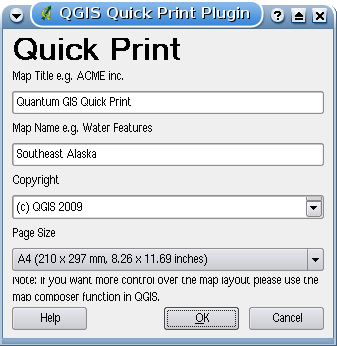
\includegraphics[clip=true, width=6cm]{quick_print_dialog}
\end{center}
\end{figure}

\begin{figure}[ht]
   \begin{center}
   \caption{Resultado de Impresión Rápida como DIN A4 PDF usando el conjunto de datos de ejemplo de alaska \nixcaption}\label{fig:quickprint_result}\smallskip
   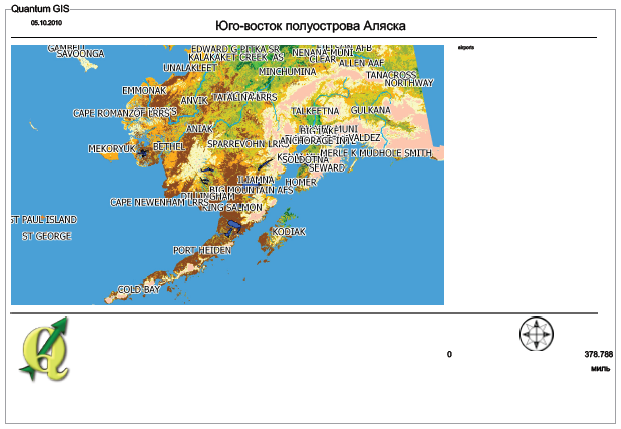
\includegraphics[clip=true, width=9cm]{quick_print_result}
\end{center}
\end{figure}
